\documentclass{beamer}

\usepackage{amsmath,amssymb,amsfonts}
\usepackage{bibentry}
\usepackage{graphicx}
\usepackage{listings}
\usepackage[latin1]{inputenc}

\lstset{
  literate={é}{{\'e}}1
}


\lstdefinelanguage{GF}{
    morekeywords={ abstract, concrete, resource, interface, instance,
        incomplete, of, with, open,
        cat, fun, lincat, lin, oper, flags, param
    },
    morecomment=[l]{--},
    morecomment=[s]{\{-}{-\}},
    morestring=[b]",
    basicstyle=\footnotesize\rmfamily
}

\lstdefinelanguage{GFcmd}{
    morekeywords={parse, linearize, view_tree},
    morestring=[b]",
    basicstyle=\footnotesize\rmfamily
}

\def\str#1{``\emph{#1}''}   % Examples in natural language
\def\log#1{{\bfseries#1}}              % Examples in logical representation

\title{Syntactic/Semantic Analysis for High-Precision Math Linguistics}
\subtitle{CICM 2018}
\author{Jan Frederik Schaefer \and Michael Kohlhase}
\institute{Friedrich-Alexander-Universit\"at Erlangen-N\"urnberg}
\date{\today} 

\usetheme{Pittsburgh}
\usecolortheme{beaver}

\begin{document}

\frame{\titlepage}

\section{Introduction}

\frame{
    \frametitle{Example}
    \str{A positive integer $n$ is called prime, iff there is no integer $1 < m < n$ such that $m | n$}

    \vspace{1em}
    \textbf{Translation to (from) German:}
    \vspace{0.2em}

    \str{Eine positive ganze Zahl $n$ ist prim genau dann, wenn es keine ganze Zahl $1 < m < n$ gibt, sodass $m | n$}

    \vspace{1em}
    \textbf{Formalization:}
    \vspace{0.2em}

%    \log{$( \forall n . ( ( \lambda x. \text{pos} ( x ) \land \text{int} ( x ) ) n ) \Rightarrow ( ( \lambda x. \text{prime} ( x ) ) n \Leftrightarrow ( \lnot \exists m . ( \lambda x. \text{int} ( x ) ) m \land \text{less} ( 1 , m ) \land \text{less} ( m , n ) \land ( \text{divides} ( m , n ) ) ) ) )$}
%    {\large $$\downarrow_\beta$$}
    \log{$\forall n . \text{pos} ( n ) \land \text{int} ( n ) \Rightarrow ( \text{prime} ( n ) \Leftrightarrow \lnot \exists m . \text{int} ( m ) \land \text{divides} ( m , n ) \land \text{less} ( 1 , m ) \land \text{less} ( m , n ) )$}
}

\frame{
    \frametitle{GF - Grammatical Framework}
    \begin{itemize}
        \item ``A programming language for multilingual grammar applications''
        \item Natural language as formal language $\Rightarrow$ limited coverage but high precision
        \item Idea:
            \begin{itemize}
                \item \emph{Abstract grammar} describes ``meaning'' we want to express
                \item \emph{Concrete grammars} describe how this is expressed in English/German/Logic/...
            \end{itemize}
    \end{itemize}
}


\frame{
    \frametitle{Abstract Grammar}
    \lstinputlisting[language=GF]{gfexample/Math.gf}

    \vspace{1em}
    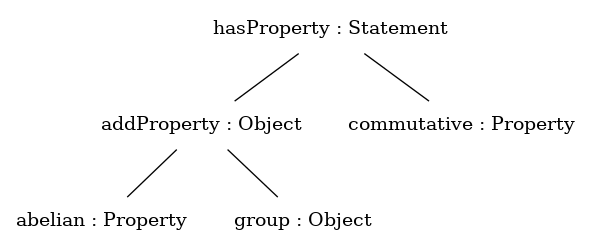
\includegraphics[scale=0.4]{trees/ab-gr_t.png}
}

\frame{
    \frametitle{Abstract Grammar}
    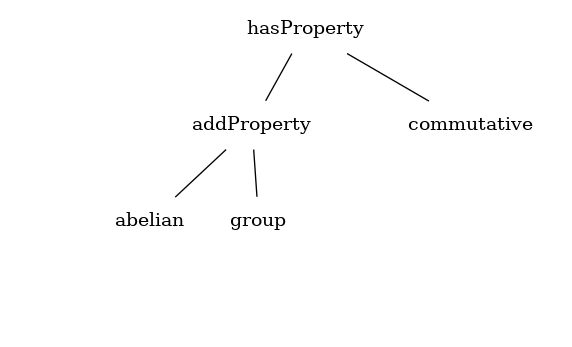
\includegraphics[scale=0.4]{trees/ab-gr-str_p_partial.png}
}

\frame{
    \frametitle{Concrete Grammar}
    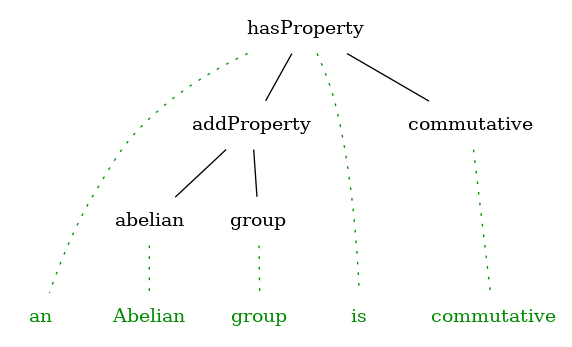
\includegraphics[scale=0.4]{trees/ab-gr-str_p.png}
}

\frame{
    \frametitle{Concrete Grammar - Simple Approach}
    \lstinputlisting[language=GF]{gfexample/MathStr.gf}

    \vspace{1em}
    Problem: \str{a} vs \str{an}
}

\frame{
    \frametitle{Concrete Grammar - Simple Approach}
    Problem: \str{a} vs \str{an}
    \begin{itemize}
        \item Idea: Use record types
        \item This is a common problem $\leadsto$ GF's \emph{resource grammar library}
    \end{itemize}
}

\frame{
    \frametitle{Concrete Grammar - Resource Grammar Library}
    \lstinputlisting[language=GF,basicstyle=\scriptsize]{gfexample/MathEng.gf}
}

\frame{
    \frametitle{Concrete Grammar - Resource Grammar Library}
    \lstinputlisting[language=GF,basicstyle=\scriptsize]{gfexample/MathFre.gf}
}

\frame{
    \frametitle{Concrete Grammar - Translation}
    
    \centering
    
    \str{un groupe ab{\'e}lien est commutatif} 
    \vspace{1em}

    {\large $\downarrow$} 
    \vspace{1em}

    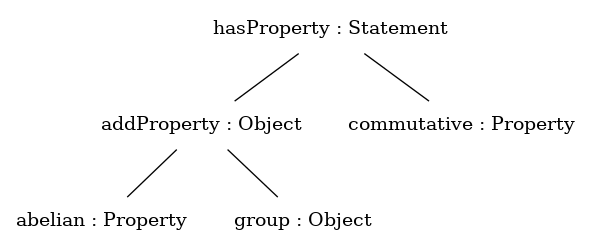
\includegraphics[scale=0.4]{trees/ab-gr_t.png} 
    \vspace{1em}

    {\large $\downarrow$} 
    \vspace{1em}

    \str{an Abelian group is commutative}
}



\frame{
    \frametitle{Using GF for Mathematics - Challenges}
    \begin{itemize}
        \item Parsing formulae
        \item Different grammatical roles of formulae in a sentence
            \begin{itemize}
                \item \str{if $n > 1$}
                \item \str{if $n + k$ is even}
            \end{itemize}
        \item Other idiosyncracies in mathematical language not covered by the resource grammar library, like
            \begin{itemize}
                \item \str{let $n$ be a\ldots}
                \item \str{an integer is called prime iff\ldots}
            \end{itemize}
        \item Finding the right abstract grammar (syntactic vs semantic)
    \end{itemize}
}

\frame{
    \frametitle{Using GF for Mathematics - Formula as Statement}
    \str{we know that $ n > 2$}
    
    \vspace{1em}
    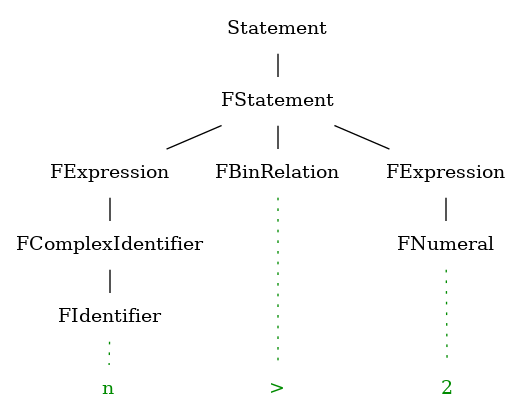
\includegraphics[scale=0.4]{trees/ng2_stmt.png}
}

\frame{
    \frametitle{Using GF for Mathematics - Formula as Identifier}
    \str{let $n > 2$ be an integer}
    
    \vspace{1em}
    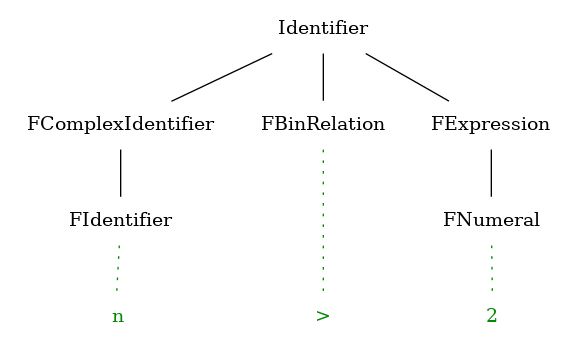
\includegraphics[scale=0.4]{trees/ng2_id.png}
}

\frame{
    \frametitle{Using GF for Mathematics - Using Identifier in Statement}
    \str{there is an integer $n$ such that \ldots}

    \vspace{1em}
    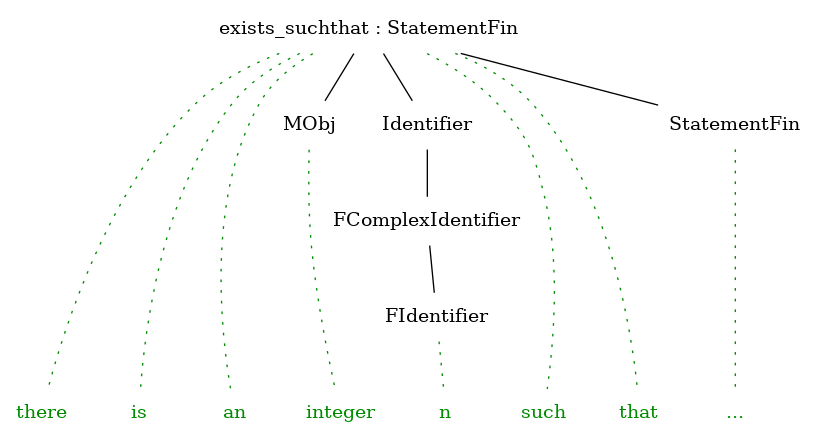
\includegraphics[scale=0.4]{trees/exn-eng_p.png}
}

\frame{
    \frametitle{Using GF for Mathematics - Using Identifier in Statement}
    \str{there is an integer $n$ such that \ldots}

    \vspace{1em}
    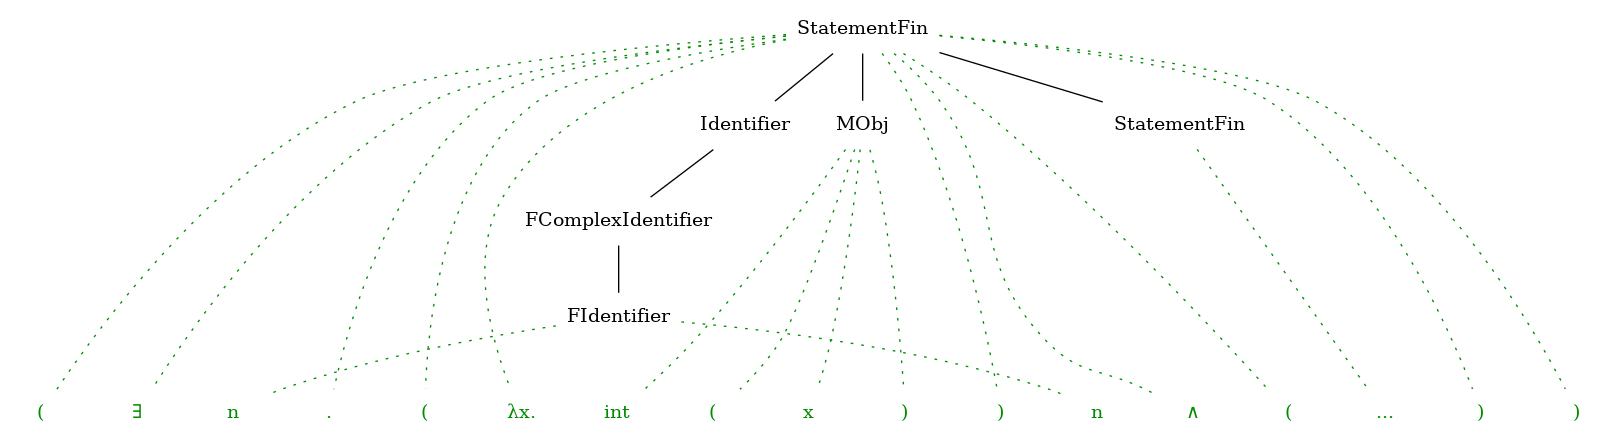
\includegraphics[scale=0.2]{trees/exn-log_p.png}

    \vspace{1em}
    \log{$(\exists n . ( \lambda x . \text{int} ( x ) ) n \land (\ldots))$}

    \vspace{1em}
    $\downarrow_\beta$
    \vspace{1em}

    \log{$\exists n . \text{int} ( n ) \land \ldots$}
}

\frame{
    \frametitle{Using GF for Mathematics - Example}
    \str{A positive integer $n$ is called prime, iff there is no integer $1 < m < n$ such that $m | n$}

    \vspace{1em}
    \textbf{Translation to (from) German:}
    \vspace{0.2em}

    \str{Eine positive ganze Zahl $n$ ist prim genau dann, wenn es keine ganze Zahl $1 < m < n$ gibt, sodass $m | n$}

    \vspace{1em}
    \textbf{Formalization:}
    \vspace{0.2em}

    \log{$( \forall n . ( ( \lambda x. \text{pos} ( x ) \land \text{int} ( x ) ) n ) \Rightarrow ( ( \lambda x. \text{prime} ( x ) ) n \Leftrightarrow ( \lnot \exists m . ( \lambda x. \text{int} ( x ) ) m \land \text{less} ( 1 , m ) \land \text{less} ( m , n ) \land ( \text{divides} ( m , n ) ) ) ) )$}
    {\large $$\downarrow_\beta$$}
    \log{$\forall n . \text{pos} ( n ) \land \text{int} ( n ) \Rightarrow ( \text{prime} ( n ) \Leftrightarrow \lnot \exists m . \text{int} ( m ) \land \text{divides} ( m , n ) \land \text{less} ( 1 , m ) \land \text{less} ( m , n ) )$}
}

\frame{
    \frametitle{Next Steps}

    \begin{itemize}
        \item Extend grammars for larger coverage
        \item Extend lexica for larger coverage
        \item Switch to DRT
    \end{itemize}
}


\end{document}
